\documentclass[11pt]{article}
\usepackage[utf8]{inputenc}
\usepackage[T1]{fontenc}
\usepackage{lmodern}
\usepackage[margin=1in]{geometry}
\usepackage{microtype}
\usepackage{graphicx}
\usepackage{booktabs}
\usepackage{array}
\usepackage{tabularx}
\usepackage{longtable}
\usepackage{float}
\usepackage{placeins}
\usepackage{xcolor}
\usepackage{caption}
\usepackage{natbib}
\usepackage[hidelinks]{hyperref}
\usepackage{fancyhdr}
\setlength{\parindent}{0pt}
\setlength{\parskip}{0.65em}
\setlength{\headheight}{14.5pt}
\renewcommand{\arraystretch}{1.15}
\definecolor{ink}{HTML}{19324A}
\definecolor{accent}{HTML}{A64B2A}
\hypersetup{colorlinks=true,linkcolor=ink,citecolor=accent,urlcolor=accent}
\pagestyle{fancy}
\fancyhf{}
\lhead{Chile BOP-Binding Progress Report v6}
\rhead{Endogenous ECT-TVECM}
\cfoot{\thepage}
\title{\textbf{Chile's Balance-of-Payments Constraint and Machinery Accumulation}\\
\large Progress report v6: endogenous import-ECT threshold VECM, 1920--2024}
\author{Chapter 2 research pipeline}
\date{29 July 2026}
\begin{document}
\maketitle

\begin{abstract}
Machinery accumulation and imports share a long-run relation in Chile that is remarkably stable across the country's central political-economic break: the machinery elasticity of imports runs from 0.83 to 0.85 across 1920--2024, 1920--1973, and 1974--2024. The adjustment to that relation is not. This report fits an endogenous error-correction threshold VECM in which the import ECT selects its own regime boundary, and finds no statistically significant asymmetry. The Hansen--Seo bootstrap does not reject linear adjustment in any sample ($p=0.374$, $0.0721$, and $0.852$), and the Seo no-cointegration test rejects nothing. The linear VECM is therefore the specification for inference, and the estimated ECT regimes are exploratory screening devices. A dating audit of the error-correction path establishes a second negative result: with each deviation dated to the year it was measured, the triangulated chronology does not identify the officially documented 1961 balance-of-payments crisis as a confirmed binding episode in either sample \citep{bcch2025}. The false negative that disqualified the previous screen survives.

\vspace{0.5em}\noindent\textbf{Keywords:} Chile; balance of payments; imports; machinery accumulation; threshold VECM; error correction; Kaldor; Thirlwall
\end{abstract}

\FloatBarrier
\section*{Resumen}
La acumulación de maquinaria y las importaciones comparten una relación de largo plazo notablemente estable en Chile: la elasticidad maquinaria--importaciones va de 0.83 a 0.85 en las tres muestras. El ajuste a esa relación no lo es. El modelo TVECM con umbral endógeno sobre el ECT no encuentra asimetría estadísticamente significativa: el bootstrap de Hansen--Seo no rechaza linealidad en ninguna muestra. El VECM lineal es la especificación válida para inferencia y los regímenes del ECT son instrumentos exploratorios de tamizaje. Una auditoría de fechamiento del ECT aporta un segundo resultado negativo: al fechar cada desviación en el año en que se midió, la cronología triangulada no identifica la crisis de balanza de pagos de 1961 como episodio confirmado en ninguna muestra. El falso negativo del tamizaje anterior persiste.

\FloatBarrier
\section{Introduction}

Chile's industrialization made foreign exchange a condition of productive transformation. Machinery and intermediate imports built the productive apparatus; weak export earnings periodically withdrew the means to pay for them \citep{bcch2025,alvarez2003}. This report examines whether the adjustment of imports to their machinery-implied long-run requirement switches between a binding and a slack regime, and whether that switch dates the periods when the external constraint actually bound.

The long-run relation survives every test put to it. The machinery elasticity of imports is 0.83--0.85 and barely moves across the 1973/74 break, which is a strong result for a peripheral economy whose trade regime, exchange-rate rule, and industrial policy were all rebuilt in between. The threshold does not survive. With the regime boundary estimated jointly with the cointegrating vector rather than imposed, the Hansen--Seo bootstrap fails to reject linear adjustment in all three samples, and the Seo no-cointegration test rejects nothing anywhere. The asymmetry that motivated the specification is not in the data at conventional significance.

That verdict sets the evidential status of everything downstream. The linear VECM carries inference. The ECT regimes remain useful as a screening layer for organizing evidence, and they are reported as such---never as estimated policy states.

The chronology built on those regimes fails its external test. The 1961 balance-of-payments crisis recorded in the Banco Central's centennial history registers as observed external pressure without the machinery-ECT signal, in the full sample and in the pre-1974 sample alike \citep{bcch2025}. That is the same false negative that disqualified the previous reduced-system screen, and it is worth being precise about how it was found: an intermediate version of this chronology did appear to capture 1961, and the appearance was an artifact of dating each error-correction value by the year of the equation it entered rather than the year of the deviation it measured. Section~\ref{sec:dating} reports the audit that caught the one-year displacement.

\FloatBarrier
\section{Mechanism and identification}

Kaldor's mechanism runs from manufacturing expansion to increasing returns and productivity growth, and cumulative causation then makes productive structure path dependent \citep{kaldor1967,kaldor1970}. Cross-country evidence supports the general manufacturing-growth mechanism without identifying a Chilean coefficient \citep{marconi2016}. Thirlwall's closure makes sustained growth conditional on export earnings and the income elasticity of imports, and later extensions admit capital flows and debt service \citep{thirlwall1979,thirlwall1982,morenobrid2003}. The theory predicts a foreign-exchange constraint on transformation. It does not predict a particular integration order, cointegrating rank, or crisis classifier, and this report does not let it substitute for one.

For Chile the connecting mechanism is imported productive inputs. Official history records that CORFO-led industrialization raised capital- and intermediate-goods imports from the late 1940s while export stagnation left insufficient foreign exchange, producing the 1961 balance-of-payments crisis \citep{bcch2025}. Plant-level analysis emphasizes technology embodied in imported capital and intermediate goods and their limited domestic substitutability \citep{alvarez2003}. The post-1974 split is equally substantive: trade reform changed manufacturing composition and productivity, import penetration weakened domestic interindustry linkages, and development remained tied to copper and externally exposed structural change \citep{ffd1983a,ffd1983b,ffd2002,albala2006,palma2019,solimano2024}. A direct Chilean application of balance-of-payments-constrained growth covers 1980--2019 and cannot adjudicate the earlier system or the 1961 benchmark \citep{yunga2022}.

\FloatBarrier
\section{Methodology}

\subsection{Data and provenance}

Every estimate consumes the frozen release \texttt{chile\_bop\_binding\_v1\_1}, 1920--2024, 105 annual observations, with 54 years before 1974 and 51 after. No stage in this report re-queries a source, re-splices a series, or reconstructs a variable. GDP, imports, investment, non-reinvested surplus, and gross machinery capital are in 2003 CLP. The Banco Central RER is an arithmetic annual mean of monthly observations, rebased from its 1986 reference to the ClioLab 2003 scale.

\begin{table}[H]
\centering
\caption{Provenance, units, and the RER splice audit}
\label{tab:provenance}
\begin{tabular}{p{6.0cm}p{2.4cm}p{5.6cm}}
\toprule
\textbf{Audit object} & \textbf{Result} & \textbf{Verdict} \\
\midrule
Price base, all real series & 2003 CLP & Matches the GDP source exactly; no rebasing applied. \\
Overlap level correlation, 1986--2010 & 0.825 & Clears the declared 0.80 floor; the definitions are related, not identical. \\
Overlap growth correlation, 1987--2010 & 0.750 & Common annual movement supports a documented splice. \\
Median absolute level gap & 9.34\% & Material, and retained in the sensitivity analysis. \\
2011 boundary log growth & 0.133 & Within four overlap-growth standard deviations. \\
Spliced annual coverage & 105 years & One row per year, 1920--2024. \\
\bottomrule
\end{tabular}
\end{table}

The splice passes every declared audit and is not seamless. The measured source gap stays in the sensitivity analysis rather than being described away.

\begin{figure}[H]
\centering
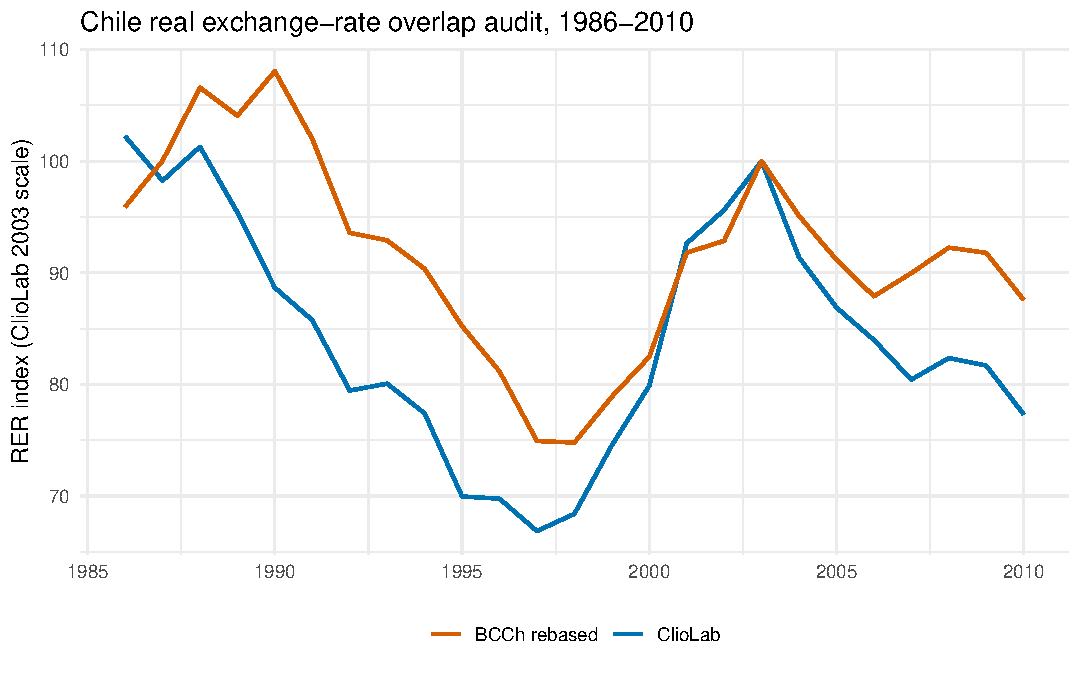
\includegraphics[width=0.92\textwidth]{figures/rer_overlap.pdf}
\caption{ClioLab and Banco Central RER over the 1986--2010 overlap.}
\end{figure}

\begin{figure}[H]
\centering
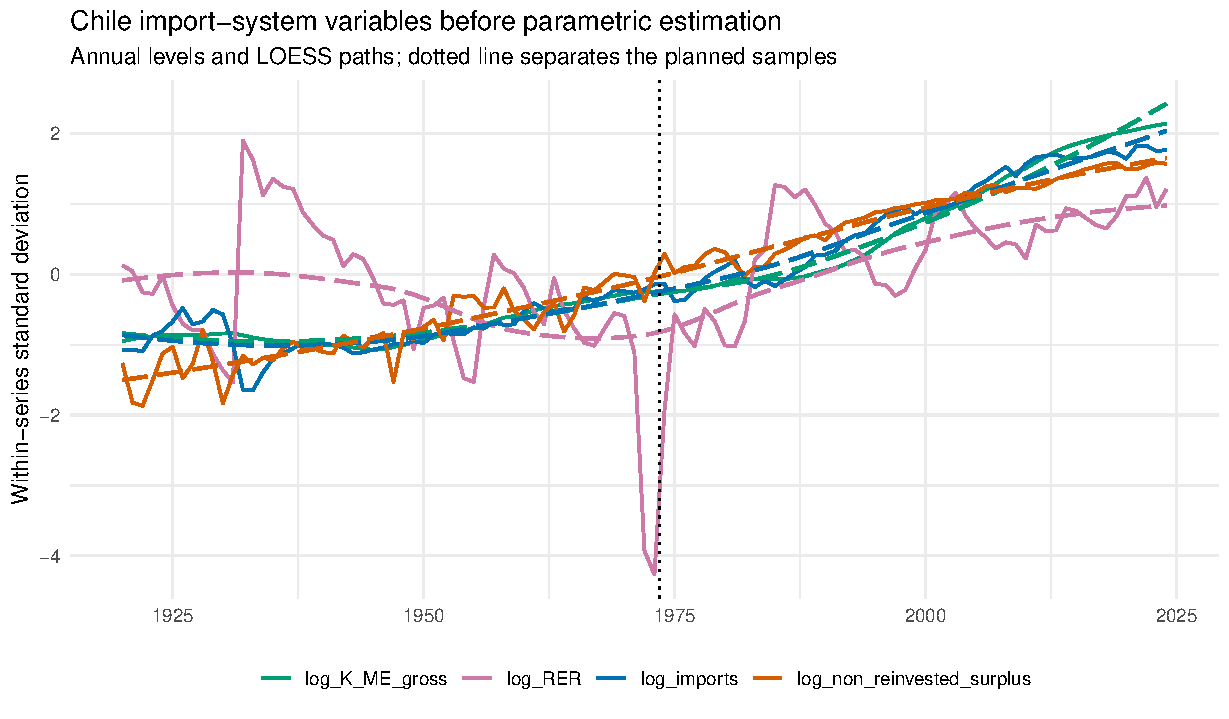
\includegraphics[width=0.96\textwidth]{figures/raw_system.pdf}
\caption{Raw import system with LOESS trends, before any parametric restriction.}
\end{figure}

\FloatBarrier
\subsection{Integration-order gate}

A sequential ADF, Phillips--Perron, and KPSS battery classifies each candidate on levels and successive differences before any long-run system is fitted. Imports and the real exchange rate are I(1) in every sample, which admits them. Gross machinery capital is I(2) in every sample, which does not. The wage share $\omega_t$ is stationary before 1974 and after 1974 and unresolved over the full span, so it enters as a control and never as a cointegrating state.

\begin{table}[H]
\centering
\caption{Sequential integration-order verdict}
\label{tab:integration}
\begin{tabular}{p{2.0cm}p{5.7cm}p{2.4cm}p{4.0cm}}
\toprule
\textbf{Sample} & \textbf{Variable} & \textbf{Classification} & \textbf{Disposition} \\
\midrule
1920--2024 & \texttt{log\_K\_ME\_gross} & I(2) & break aware or exploratory route required \\
1920--2024 & \texttt{log\_RER} & I(1) & cointegrating state candidate \\
1920--2024 & \texttt{log\_imports} & I(1) & cointegrating state candidate \\
1920--2024 & \texttt{log\_non\_reinvested\_surplus} & I(1) & cointegrating state candidate \\
1920--2024 & \texttt{wage\_share} & unresolved by d3 & break aware or exploratory route required \\
1920--1973 & \texttt{log\_K\_ME\_gross} & I(2) & break aware or exploratory route required \\
1920--1973 & \texttt{log\_RER} & I(1) & cointegrating state candidate \\
1920--1973 & \texttt{log\_imports} & I(1) & cointegrating state candidate \\
1920--1973 & \texttt{log\_non\_reinvested\_surplus} & I(0) & stationary control candidate \\
1920--1973 & \texttt{wage\_share} & I(0) & stationary control candidate \\
1974--2024 & \texttt{log\_K\_ME\_gross} & I(2) & break aware or exploratory route required \\
1974--2024 & \texttt{log\_RER} & I(1) & cointegrating state candidate \\
1974--2024 & \texttt{log\_imports} & I(1) & cointegrating state candidate \\
1974--2024 & \texttt{log\_non\_reinvested\_surplus} & I(1) & cointegrating state candidate \\
1974--2024 & \texttt{wage\_share} & I(0) & stationary control candidate \\
\bottomrule
\end{tabular}
\end{table}

The machinery result is the binding constraint on the whole exercise. A gross capital stock is an accumulated path of investment flows, so it inherits an extra unit root when those flows are themselves persistent. The theory says machinery accumulation drives the import requirement; the stochastic evidence says this particular observable proxy is not admissible in a standard long-run regression. Theory motivates a regressor; it does not license one.

\FloatBarrier
\subsection{Break-aware machinery route}

Rather than abandon the machinery channel or smuggle it past the gate, the pipeline routes it through a Zivot--Andrews and Gregory--Hansen break-aware stage and labels the result exploratory. This route is reported, not promoted. No result in Section~\ref{sec:results} acquires formal status from it.

\begin{table}[H]
\centering
\caption{Break-aware machinery route}
\label{tab:route}
\begin{tabular}{p{2.3cm}p{2.2cm}p{2.2cm}p{2.8cm}p{4.2cm}}
\toprule
\textbf{Sample} & \textbf{Standard gate} & \textbf{Break} & \textbf{Model} & \textbf{Route status} \\
\midrule
1920--2024 & I(2) & 1991 & trend & exploratory break route \\
1920--1973 & I(2) & 1936 & regime trend & exploratory break route \\
1974--2024 & I(2) & 1991 & level & exploratory break route \\
\bottomrule
\end{tabular}
\end{table}

\FloatBarrier
\subsection{Endogenous ECT-threshold VECM}

The threshold model is a bivariate TVECM in log imports and log gross machinery capital, estimated with \texttt{tsDyn} over a joint grid in the cointegrating vector and the threshold, one lag, 15\% trimming, and 999 bootstrap replications. The threshold variable is the error-correction term itself, so the regime boundary is estimated rather than read off an observed indicator such as the real exchange rate. Two tests follow: the Hansen--Seo bootstrap of linear against threshold cointegration, and the Seo test of no cointegration against threshold cointegration.

\FloatBarrier
\section{Empirical results}
\label{sec:results}

\subsection{The long-run relation is stable; the regime split is not}

The machinery elasticity of imports sits at 0.828--0.846 across all three samples. A relation this stable across the 1973/74 break says the import requirement attached to machinery accumulation is a structural feature of Chilean accumulation rather than an artifact of one trade regime. Read through the surplus approach, the coefficient is the long-run foreign-exchange cost of the intensive margin of accumulation: expanding the machinery stock draws imports in near-proportion, whichever institutional settlement is in place.

\begin{table}[H]
\centering
\caption{Endogenous ECT threshold and regime-specific adjustment}
\label{tab:threshold}
\begin{tabular}{p{2.3cm}p{2.4cm}p{2.0cm}p{2.4cm}p{2.4cm}p{2.4cm}}
\toprule
\textbf{Sample} & \textbf{Machinery elasticity} & \textbf{Threshold} $\hat{\tau}$ & \textbf{Regime} $n$ & \textbf{Adj. below} $\hat{\tau}$ & \textbf{Adj. above} $\hat{\tau}$ \\
\midrule
1920--2024 & 0.830 & 0.250 & 71 / 32 & -0.249 & -0.084 \\
1920--1973 & 0.828 & -0.047 & 36 / 16 & -0.231 & -0.803 \\
1974--2024 & 0.846 & -0.279 & 8 / 41 & -0.146 & 0.155 \\
\bottomrule
\multicolumn{6}{p{15.5cm}}{\footnotesize Regime $n$ reports observations below and above $\hat{\tau}$. Adjustment coefficients are the import-equation error-correction terms in each regime.} \\
\end{tabular}
\end{table}

Two features of this table must not be over-read. First, the full-sample threshold is positive at $0.250$. The regime labelled below $\hat{\tau}$ is therefore not the negative-ECT regime: it pools genuinely negative ECT years with mildly positive ones. The chronology in Section~\ref{sec:chronology} keeps the two definitions apart, intersecting a negative ECT with the estimated lower regime rather than conflating them. Second, the post-1974 lower regime holds 8 of 49 observations. Its adjustment coefficient is not identified with any useful precision, and the sign contrast against the upper regime in that sample carries no interpretation.

\FloatBarrier
\subsection{The threshold effect is not statistically supported}

Table~\ref{tab:tests} is the result that governs the report. The Hansen--Seo bootstrap fails to reject linear adjustment in every sample. The full sample returns $p=0.374$ and the post-1974 sample $p=0.852$, neither remotely close to conventional significance. The pre-1974 sample comes nearest at $p=0.0721$, which is marginal at 10\% and not significant at 5\%.

\begin{table}[H]
\centering
\caption{Threshold tests with bootstrap Monte Carlo error}
\label{tab:tests}
\begin{tabular}{p{2.1cm}p{1.9cm}p{1.9cm}p{1.9cm}p{1.5cm}p{1.3cm}p{3.0cm}}
\toprule
\textbf{Sample} & \textbf{H--S LR} & \textbf{Boot.} $p$ & \textbf{MC s.e.} & \textbf{Seo LR} & \textbf{Seo} $p$ & \textbf{Verdict} \\
\midrule
1920--2024 & 13.473 & 0.3744 & 0.0153 & 25.439 & 1.000 & does not reject linearity \\
1920--1973 & 16.577 & 0.0721 & 0.0082 & 23.662 & 0.999 & marginal at 10\%, not at 5\% \\
1974--2024 & 9.001 & 0.8519 & 0.0112 & 13.201 & 1.000 & does not reject linearity \\
\bottomrule
\multicolumn{7}{p{15.5cm}}{\footnotesize Hansen--Seo tests linear against threshold cointegration; Seo tests no cointegration against threshold cointegration. Monte Carlo standard error is $\sqrt{\hat{p}(1-\hat{p})/999}$.} \\
\end{tabular}
\end{table}

Because these $p$-values are simulation output, the table reports their Monte Carlo standard error. With 999 replications the standard error at the pre-1974 estimate is $0.0082$, which places $p=0.0721$ about 2.7 standard errors above 0.05 and 3.4 below 0.10. The marginal reading is not an artifact of simulation noise: more replications would sharpen the estimate without moving it across either conventional boundary.

The Seo no-cointegration test reinforces the verdict from the other direction. It fails to reject its null in every sample, at $p=1.000$, $0.999$, and $1.000$. The threshold specification therefore adds nothing that linear adjustment does not already deliver, and the estimated thresholds are profile minima rather than evidence of distinct adjustment regimes.

\begin{figure}[H]
\centering
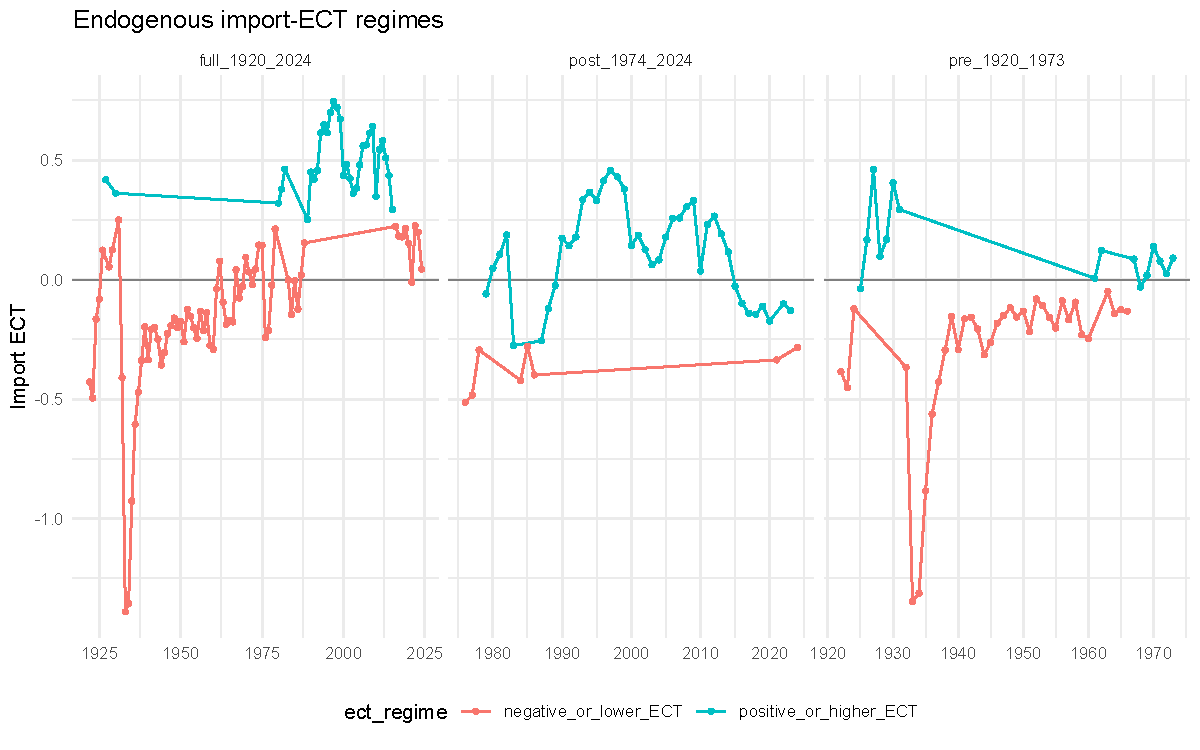
\includegraphics[width=0.92\textwidth]{figures/endogenous_ect_regimes.pdf}
\caption{Endogenous import-ECT regimes. Regime boundaries are exploratory: the Hansen--Seo bootstrap does not reject linear adjustment.}
\end{figure}

\begin{figure}[H]
\centering
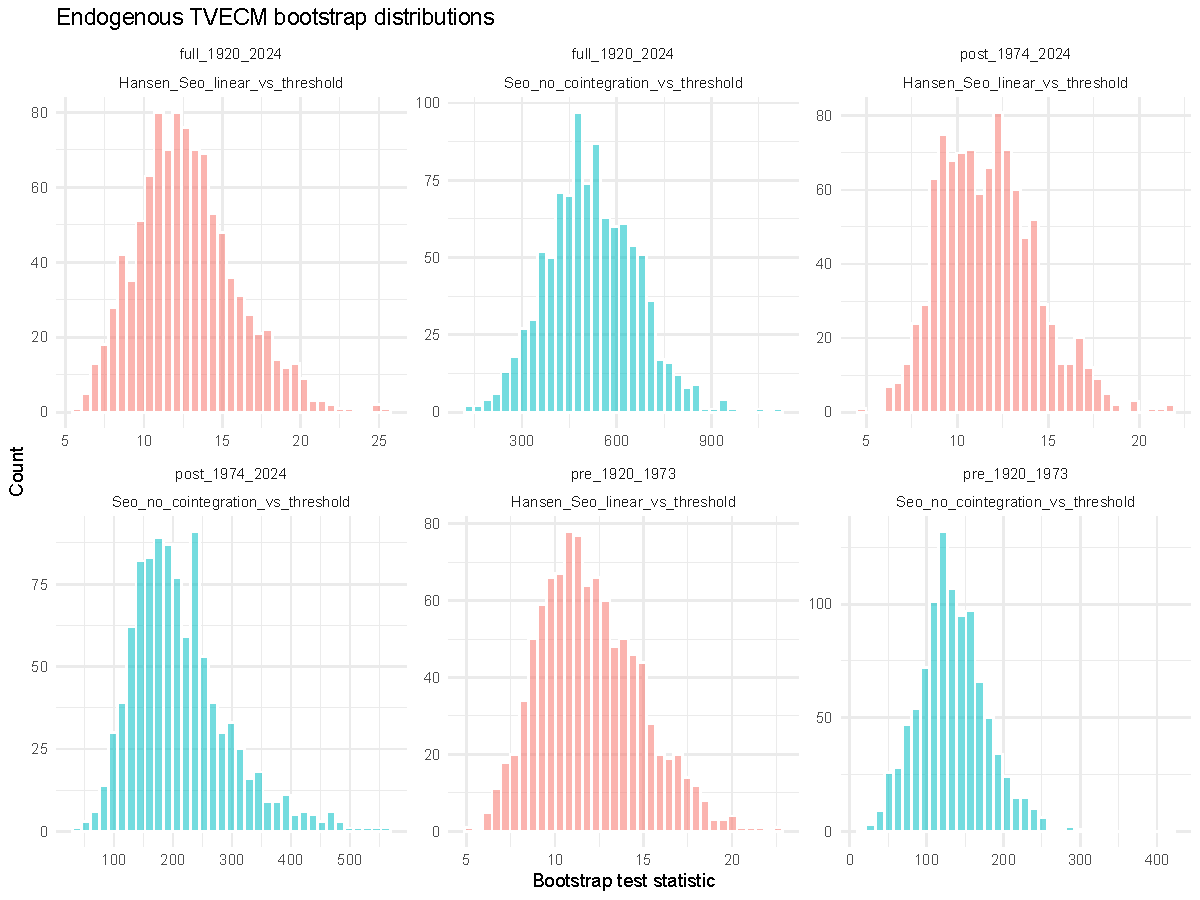
\includegraphics[width=0.92\textwidth]{figures/endogenous_tvecm_bootstrap.pdf}
\caption{Bootstrap distributions of the Hansen--Seo and Seo statistics.}
\end{figure}

\FloatBarrier
\subsection{Triangulated balance-of-payments chronology}
\label{sec:chronology}

The chronology treats the ECT regime as one of two independent requirements. A year is a confirmed binding episode only when a negative machinery-import ECT inside the estimated lower regime coincides with at least one observed external signal: a current-account or goods deficit of at least 3\% of GDP, a fall in manufactured imports of at least 3 percentage points of GDP, or the financing-compression indicator. ECT-only and observed-only years stay in separate categories, so no episode is ever confirmed by the model against itself.

\begin{table}[H]
\centering
\caption{Year classification by sample}
\label{tab:classes}
\begin{tabular}{p{2.2cm}p{2.0cm}p{1.9cm}p{2.1cm}p{1.9cm}p{1.9cm}p{1.2cm}}
\toprule
\textbf{Sample} & \textbf{Confirmed} & \textbf{ECT only} & \textbf{Observed only} & \textbf{Non-binding} & \textbf{No ECT} & \textbf{Total} \\
\midrule
1920--2024 & 28 & 21 & 26 & 28 & 2 & 105 \\
1920--1973 & 19 & 17 & 10 & 6 & 2 & 54 \\
1974--2024 & 7 & 1 & 17 & 24 & 2 & 51 \\
\bottomrule
\end{tabular}
\end{table}

The final column matters for honesty about coverage. The lag and first difference cost each sample two observations, and after the dating correction those fall at the first and last year of the sample, which therefore carry no error-correction estimate. Those years are labelled rather than silently recorded as non-binding. Every release year in every sample lands in exactly one class.

\begin{table}[H]
\centering
\caption{Confirmed binding episode runs}
\label{tab:episodes}
\begin{tabular}{p{2.6cm}p{2.4cm}p{2.2cm}p{2.2cm}p{2.6cm}}
\toprule
\textbf{Sample} & \textbf{Years} & \textbf{Duration} & \textbf{Peak year} & \textbf{Peak index} \\
\midrule
1920--2024 & 1921--1922 & 2 & 1922 & 1.728 \\
1920--2024 & 1931 & 1 & 1931 & 1.236 \\
1920--2024 & 1933 & 1 & 1933 & 1.718 \\
1920--2024 & 1937--1938 & 2 & 1938 & 0.076 \\
1920--2024 & 1949--1955 & 7 & 1954 & 0.909 \\
1920--2024 & 1957--1960 & 4 & 1958 & 0.994 \\
1920--2024 & 1962--1964 & 3 & 1963 & 0.502 \\
1920--2024 & 1971 & 1 & 1971 & 0.397 \\
1920--2024 & 1975--1977 & 3 & 1976 & 0.353 \\
1920--2024 & 1982--1985 & 4 & 1982 & 0.853 \\
1974--2024 & 1975--1977 & 3 & 1976 & 1.051 \\
1974--2024 & 1983--1985 & 3 & 1983 & 1.108 \\
1974--2024 & 2023 & 1 & 2023 & 1.248 \\
1920--1973 & 1921--1922 & 2 & 1922 & 1.960 \\
1920--1973 & 1931 & 1 & 1931 & 1.291 \\
1920--1973 & 1933 & 1 & 1933 & 3.194 \\
1920--1973 & 1937--1938 & 2 & 1938 & -0.226 \\
1920--1973 & 1949--1955 & 7 & 1954 & 0.702 \\
1920--1973 & 1957--1959 & 3 & 1958 & 0.830 \\
1920--1973 & 1962--1964 & 3 & 1963 & 0.171 \\
\bottomrule
\end{tabular}
\end{table}

\begin{figure}[H]
\centering
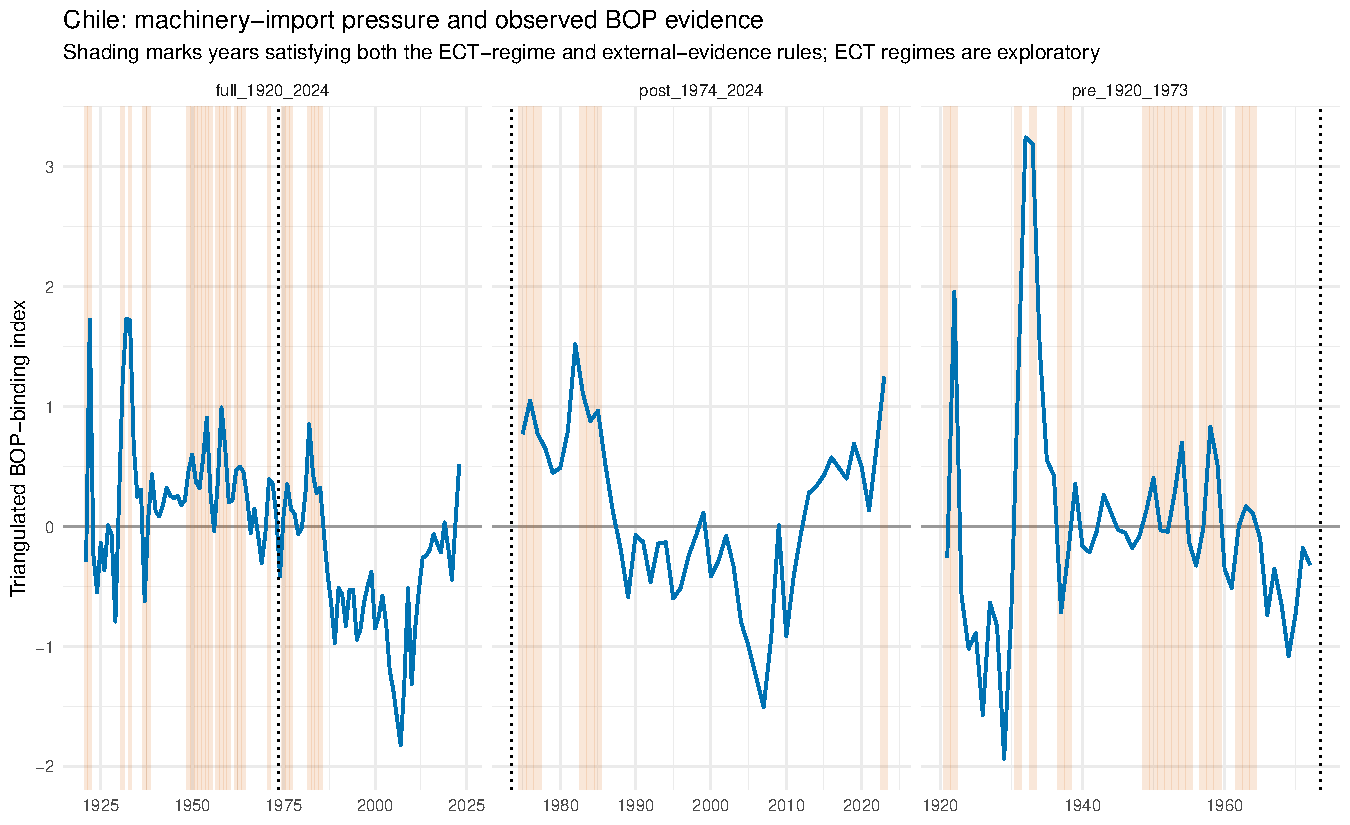
\includegraphics[width=0.92\textwidth]{figures/binding_index.pdf}
\caption{Triangulated BOP-binding index. Shading marks years satisfying both the ECT-regime and external-evidence rules.}
\end{figure}

\begin{figure}[H]
\centering
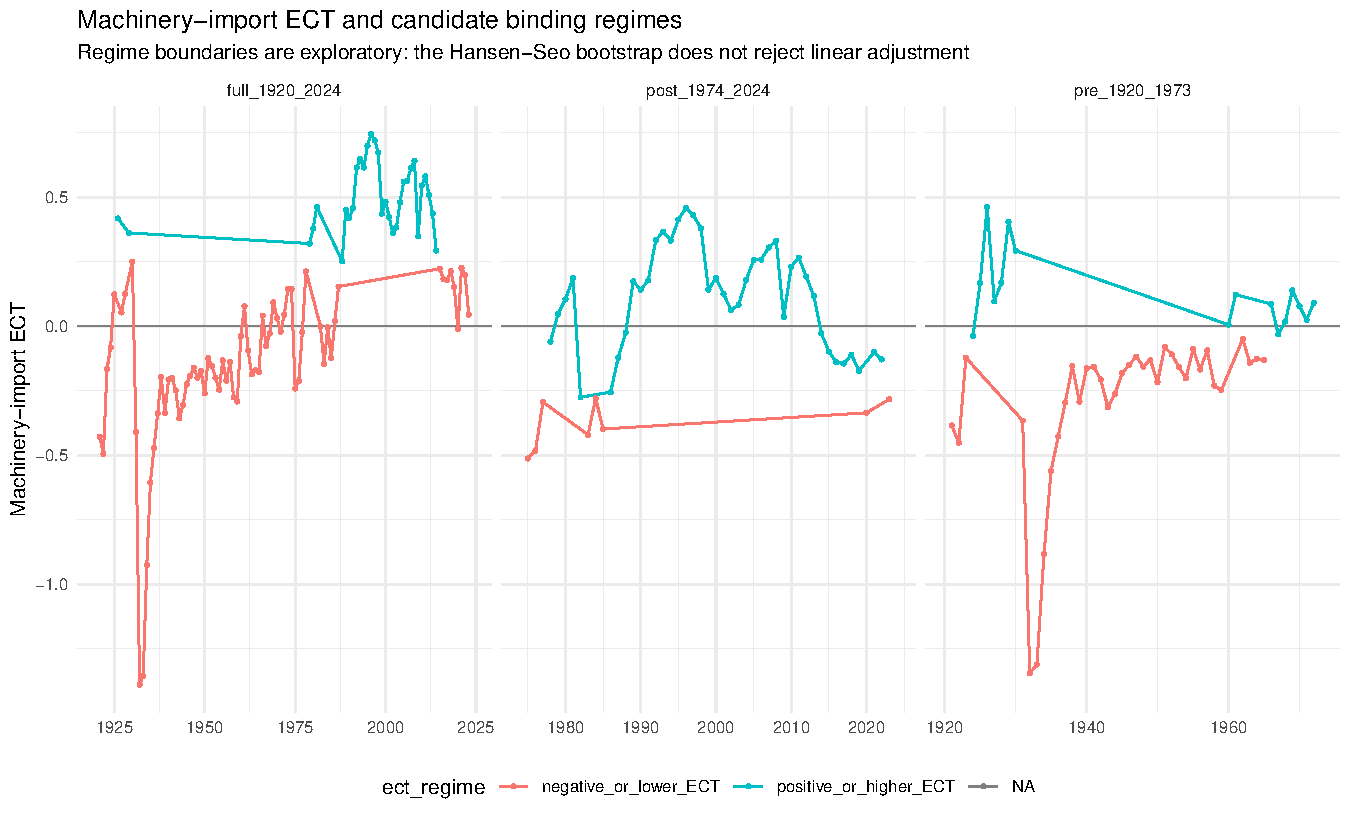
\includegraphics[width=0.92\textwidth]{figures/machinery_ect_chronology.pdf}
\caption{Machinery-import ECT chronology and candidate binding regimes.}
\end{figure}

\FloatBarrier
\subsection{Dating audit and the 1961 benchmark}
\label{sec:dating}

A threshold VECM switches regime on the lagged error-correction term: the deviation entering the year-$t$ equation is the one measured at $t-1$. That is correct for the estimator and treacherous for a chronology, because a panel that labels each deviation with the equation year attributes every disequilibrium to the year after it occurred. Triangulating such a panel against contemporaneous external indicators pairs each year's observed pressure with the previous year's model signal.

The chronology therefore does not trust the upstream year labels. It rebuilds the cointegrating relation from the frozen release using the estimated elasticity, matches it against the recorded error-correction path across a range of leads and lags, and adopts the offset that reproduces the path exactly. The audit returns a one-year displacement in all three samples, matching to a maximum absolute deviation of $1.1e-14$---machine precision, not an approximate fit. Labels are shifted back one year before any year is classified, so each deviation is dated to the year it was measured. The audit is self-checking rather than a fixed correction: if the upstream stage is re-run with corrected dating, the detected offset is zero and nothing shifts.

The consequence is the second negative result of this report. The Banco Central's centennial history records that CORFO-led industrialization raised capital- and intermediate-goods imports from the late 1940s, that export stagnation left insufficient foreign exchange, and that the sequence culminated in the 1961 balance-of-payments crisis and the abandonment of the fixed exchange rate \citep{bcch2025}. The previous reduced-system screen missed that year, and the miss was decisive against it.

\begin{table}[H]
\centering
\caption{Independent historical benchmark}
\label{tab:benchmark}
\begin{tabular}{p{1.4cm}p{2.4cm}p{4.4cm}p{2.4cm}p{4.0cm}}
\toprule
\textbf{Year} & \textbf{Sample} & \textbf{Model classification} & \textbf{Binding index} & \textbf{Agreement} \\
\midrule
1961 & 1920--2024 & observed BOP only pressure & 0.220 & captured as observed BOP only \\
1961 & 1920--1973 & observed BOP only pressure & -0.510 & captured as observed BOP only \\
\bottomrule
\end{tabular}
\end{table}

Correctly dated, the machinery-ECT chronology misses 1961 too. In both samples the year registers as observed external pressure without the machinery-ECT signal: the external evidence is present, the model signal is not. Before the dating audit the full sample appeared to capture 1961 as a confirmed binding year, and that reading was an artifact of the one-year displacement---the signal it credited to 1961 belonged to 1960. Replacing the machinery route for the reduced-system route does not repair the false negative; it relocates it.

The negative result is informative about the screen rather than about Chile. A single-equation disequilibrium measure built on machinery accumulation identifies episodes in which imports fell below their machinery-implied requirement. It is not built to identify a reserve crisis resolved by devaluation, which is what 1961 was, and which registers in the observed external accounts precisely where the chronology puts it. The screen organizes evidence; it does not date crises.

One benchmark is also a thin test. The verified evidence base for this pipeline supplies exactly one precisely dated official crisis, and no additional marker was invented to pad the comparison. A chronology that fails its only external test has not been rescued by the size of the test set.

\FloatBarrier
\section{What remains unresolved}

\textbf{Machinery's integration order.} Gross machinery capital is I(2) under the standard gate in all three samples. The break-aware route is exploratory, and it stays exploratory: no result in this report acquires formal status from it. Until the stock's stochastic properties are resolved---by a net-stock or investment-flow formulation, or by an explicitly I(2)-admissible estimator---the machinery channel cannot carry paper-facing inference.

\textbf{The threshold effect.} Not statistically supported. The Hansen--Seo bootstrap fails to reject linearity in every sample and the Seo test rejects nothing. The pre-1974 marginal result at $p=0.0721$ is worth revisiting on a longer or higher-frequency sample; it is not worth reporting as a regime finding now.

\textbf{Three-regime inaction band.} The three-regime model was fitted and gated for feasibility, but its thresholds and coefficients were never written out, so this report records feasibility rather than a completed robustness check. The gate itself is fragile: the recorded minimum outer-regime size for the post-1974 sample is 8.33, which rounds to the eight observations the gate requires and sits exactly on its boundary. The recorded figure also scales regime shares by the pre-lag row count rather than the effective estimation sample, which is why it is not an integer. A three-regime inaction band is not evidence in this report.

\textbf{The chronology's external validity.} The screen fails its only dated external benchmark. Until it identifies 1961---or until an argument is made for why a machinery-import disequilibrium measure should not be expected to identify a reserve crisis resolved by devaluation---the episode panel is a device for organizing evidence and nothing more. The benchmark set also needs to grow before failure or success on it means much.

\textbf{RER-only external threshold.} Planned as a comparison and not yet fitted. The previous pipeline found no RER-threshold effect in reduced systems, so the comparison is expected to be negative; it has not been run on the machinery system and is not claimed either way.

\textbf{Bootstrap reproducibility.} The S40 ledgers consumed here were produced before the estimation script set a random seed. The reported bootstrap $p$-values are therefore not exactly reproducible, which is why their Monte Carlo standard errors appear in Table~\ref{tab:tests}. The script now seeds the bootstrap, so subsequent runs are reproducible and will differ from these figures within simulation error.

\FloatBarrier
\section{Next empirical decision}

The decision rule set before estimation was explicit: proceed to threshold-aware analysis if the Hansen--Seo bootstrap rejected linearity at 5\%, and treat the linear VECM as adequate otherwise. No sample rejects. The linear VECM is the specification for inference, and the threshold branch closes.

Three steps follow. Resolve machinery's integration order, since that blocks the long-run system regardless of what the adjustment dynamics turn out to be. Report the linear machinery relation alongside the ARDL fallback, with the I(2) limitation stated rather than managed. Keep the ECT chronology as a screening layer for organizing historical evidence, and extend the external benchmark set beyond 1961 so that the screen faces a real test rather than a single date.

\FloatBarrier
\section*{Data availability and reproducibility}

The frozen release is \texttt{data/releases/chile\_bop\_binding\_v1\_1/}. Every table and figure in this report is copied from a completed stage ledger; the report builder performs no estimation and records the SHA-256 hash of each consumed input in \texttt{output/CL/BOP\_BINDING\_V6/S99\_REPORT\_ASSEMBLY/}. Staged ledgers accompany the report in \texttt{data/}. Stage integrity ledgers for S30, S32, S40, and S50 all report passing checks, and the builder refuses to assemble if any of them fails.

\textbf{Ethics.} The study uses historical aggregate data and involves no human subjects.

\textbf{AI-use disclosure.} Claude Code assisted with reproducible code, diagnostics, evidence organization, and report assembly under human direction. All claims are auditable against the frozen release and the staged stage ledgers.

\FloatBarrier
\begin{thebibliography}{99}
\raggedright

\bibitem[Albala-Bertrand(2006)]{albala2006}
Albala-Bertrand, J. M. (2006). Changes in Chile's production structure, 1986--1996: Output and industrial interdependence. \textit{CEPAL Review, 88}, 159--172.

\bibitem[Álvarez and Fuentes(2003)]{alvarez2003}
Álvarez, R., \& Fuentes, J. R. (2003). \textit{Trade reforms and manufacturing industry in Chile} (Working Paper No. 210). Banco Central de Chile.

\bibitem[Banco Central de Chile(2025)]{bcch2025}
Banco Central de Chile. (2025). \textit{100 años de política económica y comercio exterior de Chile}.

\bibitem[Ffrench-Davis(1983a)]{ffd1983a}
Ffrench-Davis, R. (1983a). El experimento monetarista en Chile: Una síntesis crítica. \textit{Desarrollo Económico, 23}(90), 163--196. \url{https://doi.org/10.2307/3466468}

\bibitem[Ffrench-Davis(1983b)]{ffd1983b}
Ffrench-Davis, R. (1983b). Deuda externa y balanza de pagos de América Latina: Tendencias recientes y perspectivas. \textit{Estudios Internacionales, 16}(62), 281--304. \url{https://doi.org/10.5354/0719-3769.1983.16673}

\bibitem[Ffrench-Davis(2002)]{ffd2002}
Ffrench-Davis, R. (2002). \textit{Economic reforms in Chile: From dictatorship to democracy}. University of Michigan Press. \url{https://doi.org/10.3998/mpub.17208}

\bibitem[Kaldor(1967)]{kaldor1967}
Kaldor, N. (1967). \textit{Strategic factors in economic development}. Cornell University.

\bibitem[Kaldor(1970)]{kaldor1970}
Kaldor, N. (1970). The case for regional policies. \textit{Scottish Journal of Political Economy, 17}(3), 337--348. \url{https://doi.org/10.1111/j.1467-9485.1970.tb00712.x}

\bibitem[Marconi et al.(2016)]{marconi2016}
Marconi, N., Reis, C. F. de B., \& Araújo, E. C. de. (2016). Manufacturing and economic development: The actuality of Kaldor's first and second laws. \textit{Structural Change and Economic Dynamics, 37}, 75--89. \url{https://doi.org/10.1016/j.strueco.2015.12.002}

\bibitem[Moreno-Brid(2003)]{morenobrid2003}
Moreno-Brid, J. C. (2003). Capital flows, interest payments and the balance-of-payments constrained growth model. \textit{Metroeconomica, 54}(2--3), 346--365. \url{https://doi.org/10.1111/1467-999X.00170}

\bibitem[Palma(2019)]{palma2019}
Palma, J. G. (2019). Desindustrialización, desindustrialización ``prematura'' y ``síndrome holandés''. \textit{El Trimestre Económico, 86}(344), 901--966. \url{https://doi.org/10.20430/ete.v86i344.970}

\bibitem[Solimano and Zapata-Román(2024)]{solimano2024}
Solimano, A., \& Zapata-Román, G. (2024). \textit{Chilean economic development under neoliberalism}. Cambridge University Press. \url{https://doi.org/10.1017/9781009477352}

\bibitem[Thirlwall(1979)]{thirlwall1979}
Thirlwall, A. P. (1979). The balance of payments constraint as an explanation of international growth rate differences. \textit{PSL Quarterly Review, 32}(128), 45--53. \url{https://doi.org/10.13133/2037-3643/12804}

\bibitem[Thirlwall and Hussain(1982)]{thirlwall1982}
Thirlwall, A. P., \& Hussain, M. N. (1982). The balance of payments constraint, capital flows and growth rate differences between developing countries. \textit{Oxford Economic Papers, 34}(3), 498--510. \url{https://doi.org/10.1093/oxfordjournals.oep.a041565}

\bibitem[Yunga Medina et al.(2022)]{yunga2022}
Yunga Medina, F., Tapia Morquecho, C., Camacho Manzanillas, S., \& Cueva Jiménez, A. (2022). Does the balance of payments constrain economic growth? New evidence for Chile 1980--2019. \textit{Boletín de Coyuntura, 35}, 25--35. \url{https://doi.org/10.31243/bcoyu.35.2022.1851}

\end{thebibliography}
\end{document}

